\documentclass[a4paper]{article}
\usepackage[utf8]{inputenc}
\usepackage[spanish, es-tabla, es-noshorthands]{babel}
\usepackage[table,xcdraw]{xcolor}
\usepackage[a4paper, footnotesep=1.25cm, headheight=1.25cm, top=2.54cm, left=2.54cm, bottom=2.54cm, right=2.54cm]{geometry}
%\geometry{showframe}

%\usepackage{wrapfig}			%Wrap figure in text
\usepackage[export]{adjustbox}	%Move images
\usepackage{changepage}			%Move tables

\usepackage{tikz}
\usepackage{amsmath}
\usepackage{amsfonts}
\usepackage{amssymb}
\usepackage{float}
\usepackage{graphicx}
\usepackage{caption}
\usepackage{subcaption}
\usepackage{multicol}
\usepackage{multirow}
\usepackage{wrapfig}
\setlength{\doublerulesep}{\arrayrulewidth}
\usepackage{booktabs}
\usepackage[numbib, nottoc, notlot, notlof]{tocbibind}

\usepackage{hyperref}
\hypersetup{
    colorlinks=true,
    linkcolor=blue,
    filecolor=magenta,      
    urlcolor=blue,
    citecolor=blue,    
}

%Change Font Size

% #1 = size, #2 = text
\newcommand{\setparagraphsize}[2]{{\fontsize{#1}{6}\selectfont#2 \par}}		%Cambia el size de todo el parrafo
\newcommand{\setlinesize}[2]{{\fontsize{#1}{6}\selectfont#2}}				%Cambia el font de una oración

\newcommand{\note}[1]{
	\begin{center}
		\huge{ \textcolor{red}{#1} }
	\end{center}
}

%FONTS (IMPORTANTE): Compilar en XeLaTex o LuaLaTeX
\usepackage{anyfontsize}	%Font size
\usepackage{fontspec}		%Font type

\usepackage{etoolbox}
\usepackage{todonotes}

\newcommand{\observacion}[2]{  \ifnumequal{1}{#1}{ { \todo[inline,backgroundcolor=red!25,bordercolor=red!100]{\textbf{Observación: #2}} } }{  }  }

\setcounter{topnumber}{2}
\setcounter{bottomnumber}{2}
\setcounter{totalnumber}{4}
\renewcommand{\topfraction}{0.85}
\renewcommand{\bottomfraction}{0.85}
\renewcommand{\textfraction}{0.15}
\renewcommand{\floatpagefraction}{0.8}
\renewcommand{\textfraction}{0.1}
\setlength{\floatsep}{5pt plus 2pt minus 2pt}
\setlength{\textfloatsep}{5pt plus 2pt minus 2pt}
\setlength{\intextsep}{5pt plus 2pt minus 2pt}

\newcommand{\quotes}[1]{``#1''}
\usepackage{array}
\newcolumntype{C}[1]{>{\centering\let\newline\\\arraybackslash\hspace{0pt}}m{#1}}
\usepackage[american]{circuitikz}
\usetikzlibrary{calc}
\usepackage{fancyhdr}
\usepackage{units} 

\graphicspath{{../Control de posición no lineal/}{../Control de fuerza no lineal/}{../Control híbrido no lineal/}{../Referencias/}{../Deducción de modelo/}{../Conclusiones/}}

\pagestyle{fancy}
\fancyhf{}
\lhead{22.99 - Automación Industrial}
\rhead{Lambertucci, Londero B., Maselli, Mechoulam}
\rfoot{Página \thepage}

%Items con bullets y no cuadrados
\renewcommand{\labelitemi}{\textbullet }


\begin{document}

%%%%%%%%%%%%%%%%%%%%%%%%%
%		Caratula		%
%%%%%%%%%%%%%%%%%%%%%%%%%

\begin{titlepage}
\newcommand{\HRule}{\rule{\linewidth}{0.5mm}}
\center
\mbox{\textsc{\LARGE \bfseries {Instituto Tecnológico de Buenos Aires}}}\\[1.5cm]
\textsc{\Large 22.90  Automaci\'on Industrial}\\[0.5cm]


\HRule \\[0.6cm]
{ \Huge \bfseries Segundo Parcial}\\[0.4cm] 
\HRule \\[1.5cm]


{\large

\emph{Alumno:}\\
\vspace{3pt}

\begin{tabular}{lr} 	
\textsc{Lambertucci}, Guido Enrique  & 58009 \\

\end{tabular}

\vspace{20pt}

\emph{Profesores}\\
\textsc{Arias}, Rodolfo Enrique  \\
\vspace{3pt}
\textsc{Spinelli}, Mariano Tomás \\	
\vspace{3pt}
\textsc{Avogadro}, Federico Sofio \\	
\vspace{3pt}
\vspace{100pt}

\begin{tabular}{ll}

Presentado: & 18/11/21\\

\end{tabular}

}

\vfill

\end{titlepage}

%%%%%%%%%%%%%%%%%%%%%
%		Indice		%
%%%%%%%%%%%%%%%%%%%%%

\tableofcontents
\newpage

%%%%%%%%%%%%%%%%%%%%%
%		Informe		%
%%%%%%%%%%%%%%%%%%%%%

\section{Simulación del Carro con Péndulo Simple}

Para la simulación del carro con péndulo simple se creó un modelo de este utilizando Simscape de Simulink, utilizando una máscara para poder modificar posteriormente los siguientes parámetros:

\begin{itemize}
\item Masa del carro
\item Masa del péndulo
\item Longitud del Péndulo
\end{itemize}

\begin{figure}[H]
	\centering
	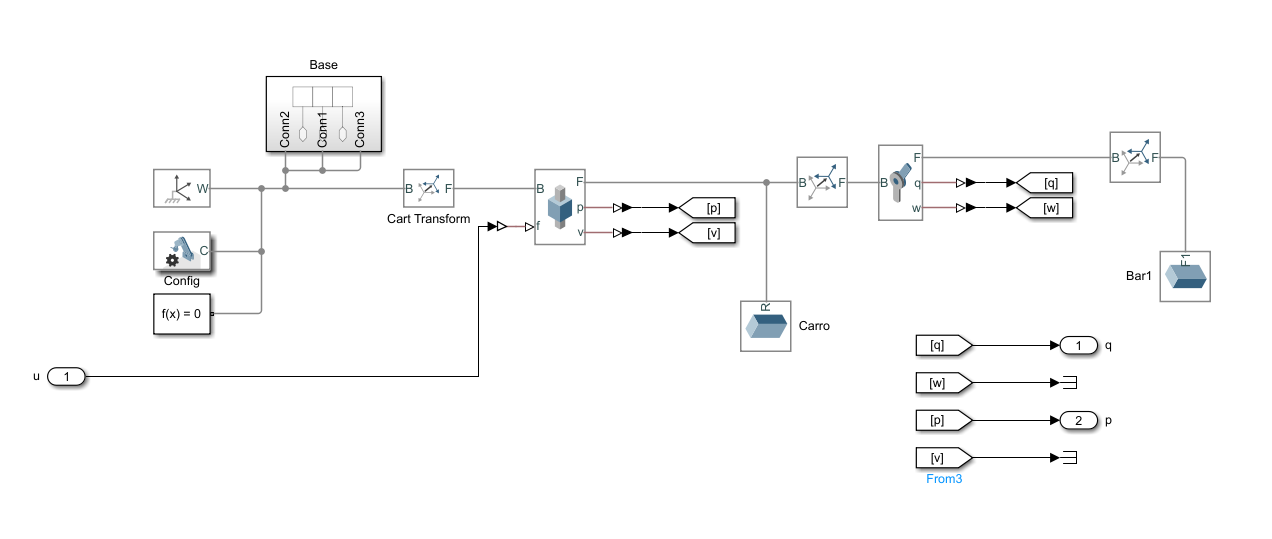
\includegraphics[width=1\linewidth]{Imagenes/loopshaping/Simscape}
	\caption{Modelo de Simscape utilizado como planta.}
	\label{1_simscape}
\end{figure}

\section{Carro con Péndulo Simple: Control en Cascada por Loop Shaping}

Para el control del sistema por loop shaping, como primer paso, se asignaron las variables del modelo de la siguiente forma:

\begin{itemize}
\item Masa del carro = $1 \ kg$
\item Masa del péndulo = $0.25 \ kg$
\item Longitud del Péndulo = $8 \ m$
\end{itemize}

Luego, se utilizó el Model Linearizer de Simulink para linealizar la planta alrededor de $q=0$, $p=0$ y $f=0$; siendo $q$ el ángulo del péndulo, $p$ la posición del carrito y $f$ la fuerza aplicada al carrito.

\begin{figure}[H]
	\centering
	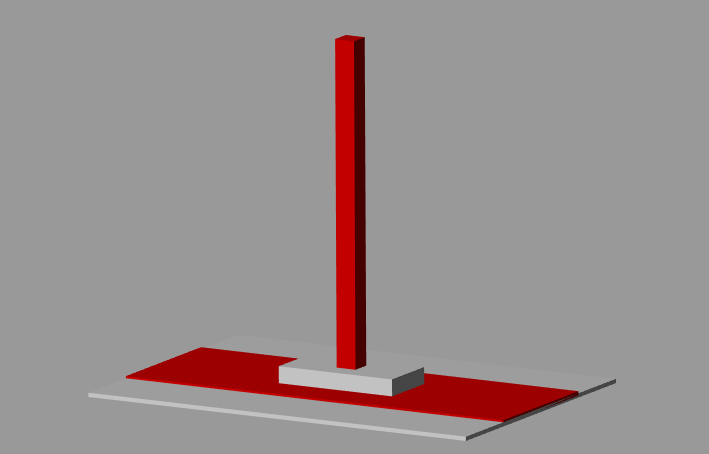
\includegraphics[width=0.5\linewidth]{Imagenes/loopshaping/equilibrio}
	\caption{Punto de equilibrio de linealización.}
	\label{1_equilibrio}
\end{figure}

\subsection{Primer Lazo: Control del Ángulo}

De esta manera, se obtuvo la siguiente transferencia desde la fuerza aplicada al carrito al ángulo del péndulo:

\begin{equation}
\frac{Q(s)}{F(s)} = \frac{0.1763}{(s-1.47)(s+1.47)}
\end{equation}

donde se nota la presencia de un polo en el semiplano derecho.

Se cierra un lazo de realimentación, tomando el valor de $q$ e inyectándolo a la entrada con una ganancia de valor $-1$ y se grafica la respuesta en frecuencia del sistema viendo solamente el ángulo $q$, obteniendo:

\begin{figure}[H]
	\centering
	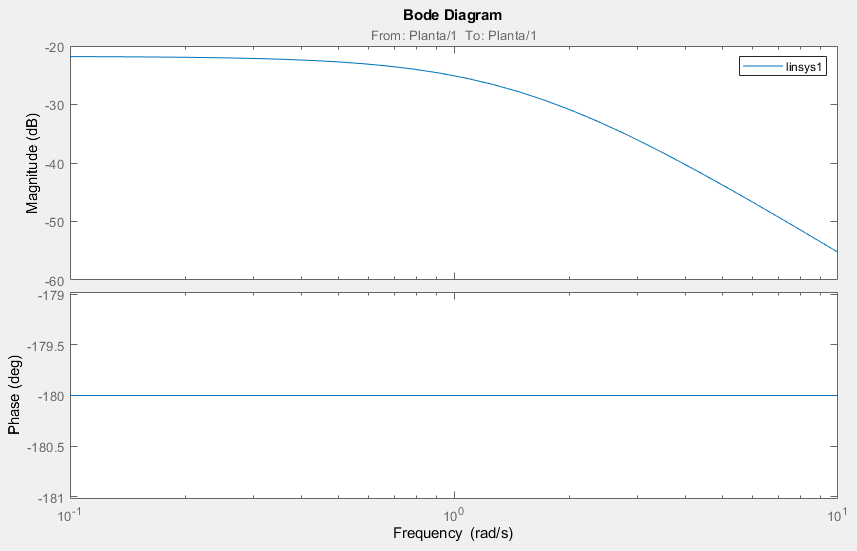
\includegraphics[width=0.8\linewidth]{Imagenes/loopshaping/bode_cerrando_q}
	\caption{Respuesta en frencuencia del sistema entre la fuerza aplicada al carrito y el ángulo del péndulo.}
	\label{bode_cerrando_q}
\end{figure}

donde se observa, como se esperaba, que el sistema es inestable. Notando el polo en el semiplano derecho en $1.47 \frac{rad}{s}$, se decide utilizar un controlador que agregue adelanto de fase para obtener una frecuencia de cruce en $w_{cruce} > 1.7 * w_{rhp} = 2.5 \frac{rad}{s}$, eligiendo entonces agregar un cero de $2.6 \frac{rad}{s}$, quedando entonces:

\begin{equation}
C_2(s) = \frac{s+2.6}{s+200}
\end{equation} 

Cabe notar que se agregó un polo rápido que no afecte la dinámica del sistema en $200 \frac{rad}{s}$ para lograr un controlador propio.

Luego, se graficó nuevamente la respuesta en frecuencia, obteniendo:

\begin{figure}[H]
	\centering
	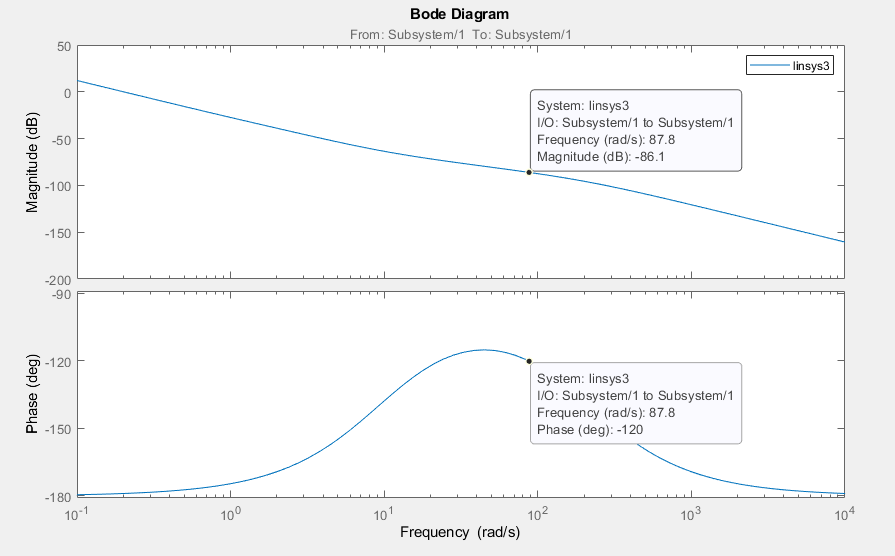
\includegraphics[width=0.8\linewidth]{Imagenes/loopshaping/bode_cerrando_q_con_controlador}
	\caption{Respuesta en frencuencia del sistema entre la fuerza aplicada al carrito y el ángulo del péndulo con controlador.}
	\label{bode_cerrando_q_con_controlador}
\end{figure}

Se busca un margen de fase de $60$ grados, por lo que se agrega una ganancia de $103 dB$ al controlador, calculado como se observa en la Figura (\ref{bode_cerrando_q_con_controlador}). Finalmente, se tiene que

\begin{equation}
C_2(s) = 1.3335e+05 \cdot \frac{s+2.6}{s+200}
\end{equation}

Se valida el control graficando una última vez la respuesta en frencuencia quedando:

\begin{figure}[H]
	\centering
	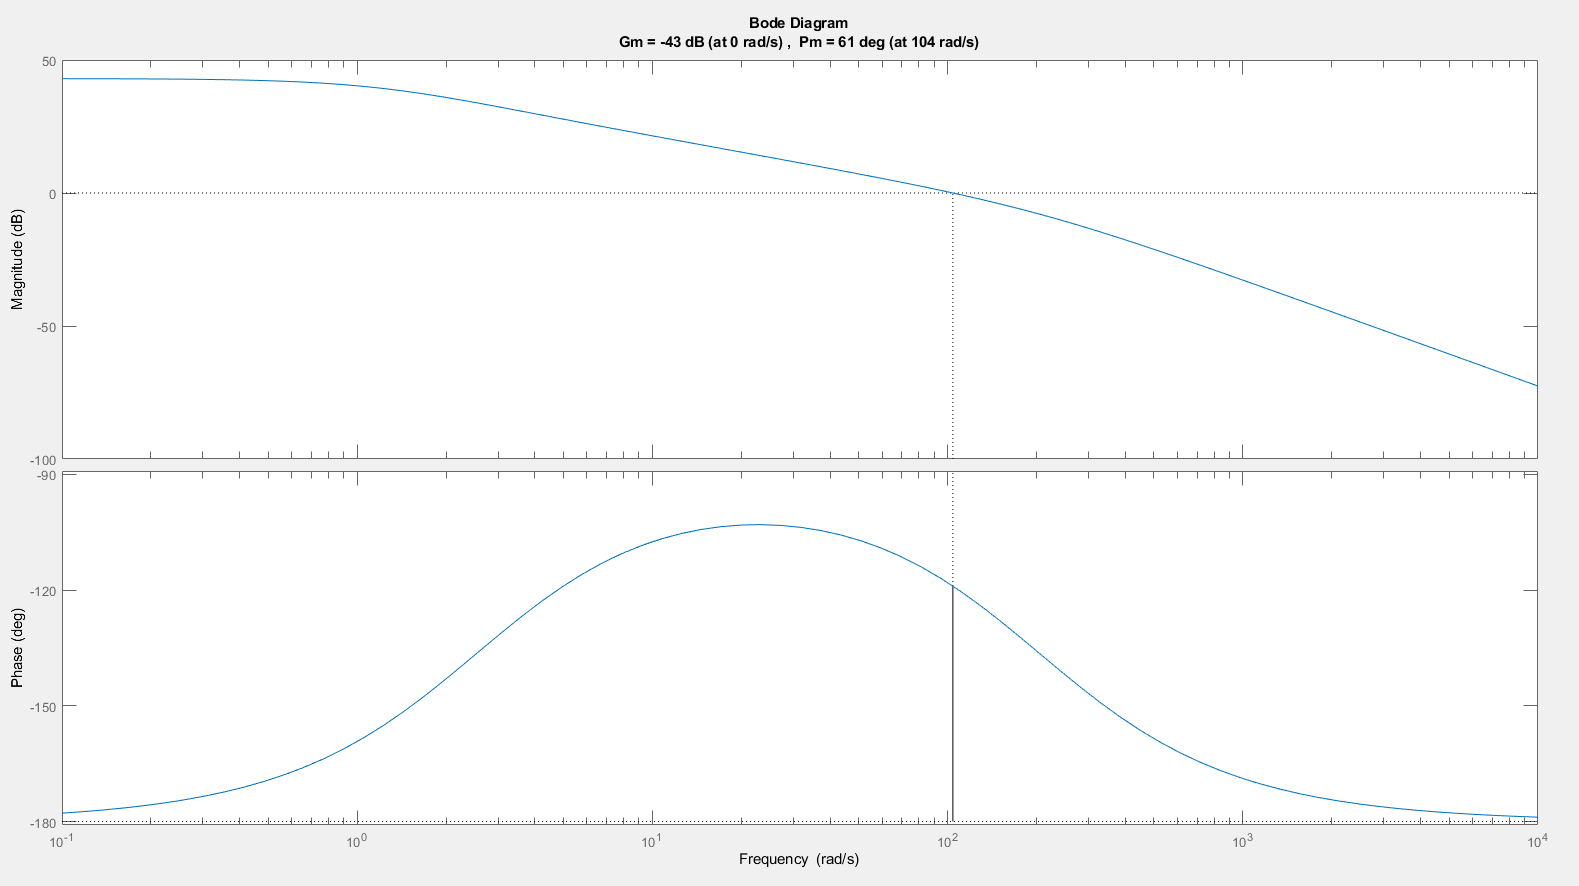
\includegraphics[width=0.8\linewidth]{Imagenes/loopshaping/bode_cerrando_q_con_controlador_ganancia}
	\caption{Respuesta en frencuencia del sistema entre la fuerza aplicada al carrito y el ángulo del péndulo con controlador y frecuencia de cruce ajustada.}
	\label{bode_cerrando_q_con_controlador_ganancia}
\end{figure}

donde se observa que el margen de fase es de $\approx 61$ grados.

En este punto del diseño, si se simula el carrito con un disturbio de ruido blanco de un segundo de frecuencia de muestreo, se puede observar que el ángulo es correctamente estabilizado, sin embargo el carrito presenta drift al no ser controlada la posición de este.

\begin{figure}[H]
	\centering
	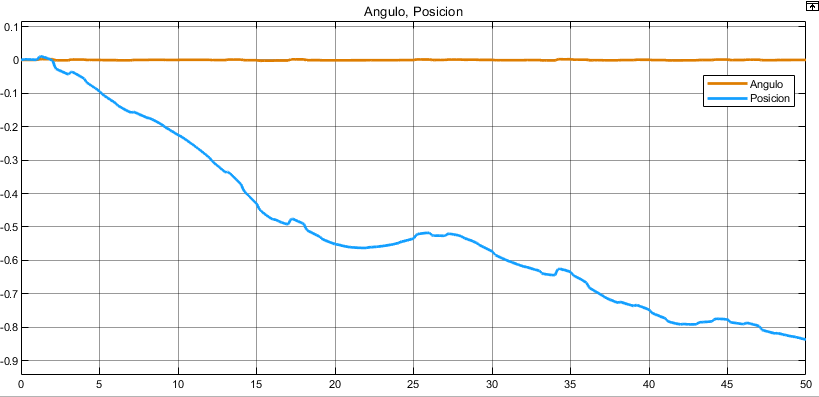
\includegraphics[width=0.8\linewidth]{Imagenes/loopshaping/simulacion_solo_angulo}
	\caption{Simulación de la planta controlando únicamente el ángulo del péndulo.}
	\label{simulacion_solo_angulo}
\end{figure}

En la Figura (\ref{s_q}) se puede observar la respuesta en frecuencia de la funcion transferencia de la sensibilidad. Se puede comprobar un buen margen de estabilidad notando que el sobrepico es de $2.38 \ dB$.

\begin{figure}[H]
	\centering
	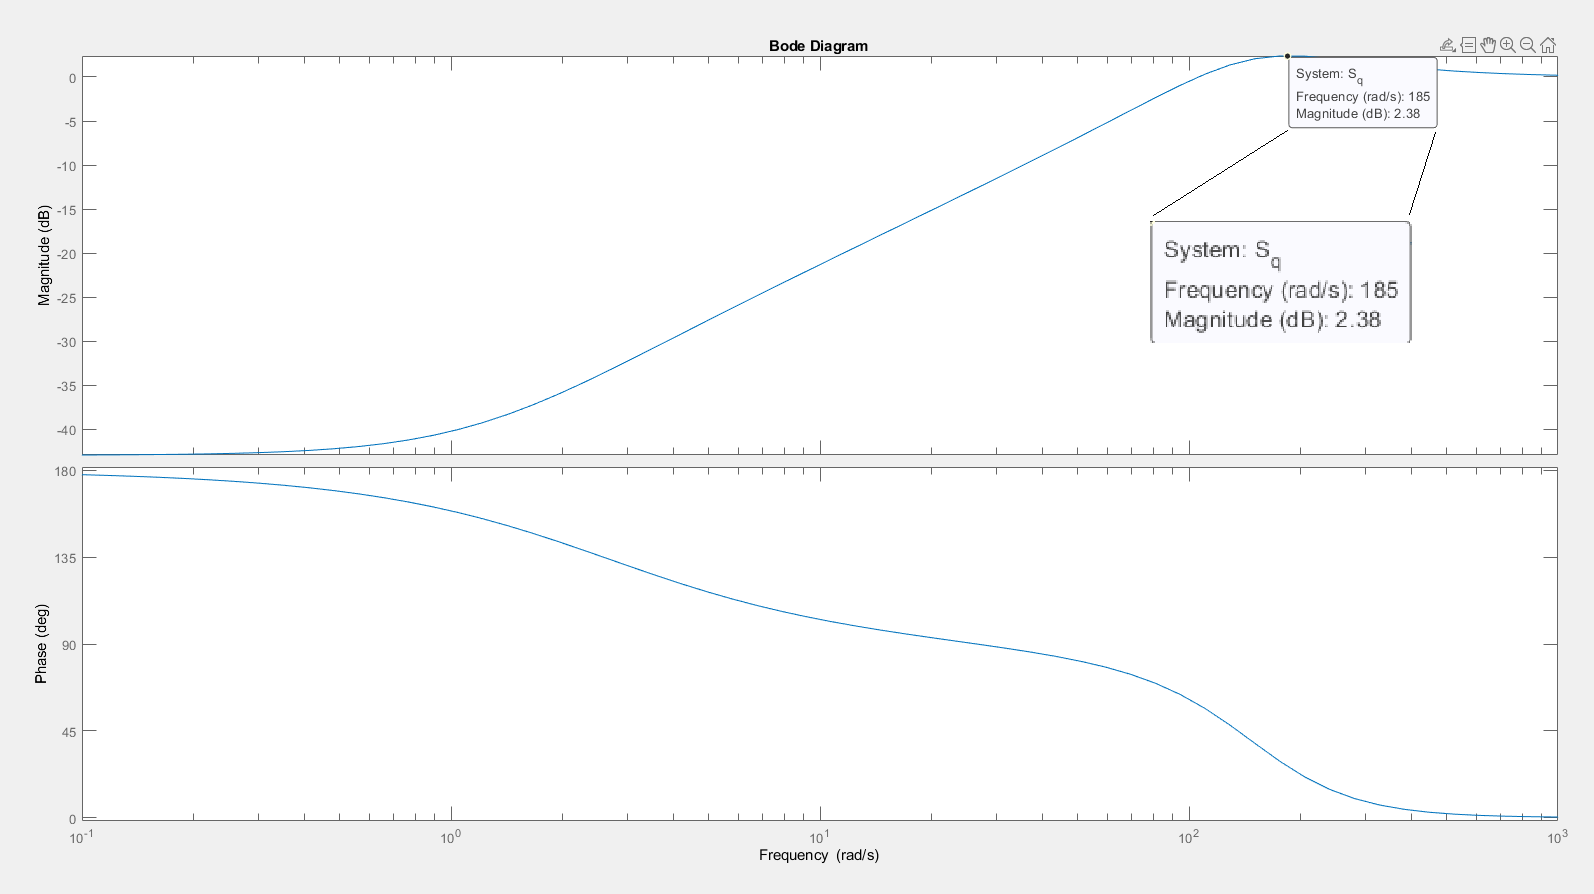
\includegraphics[width=0.8\linewidth]{Imagenes/loopshaping/bode_s_q}
	\caption{Respuesta en frecuencia de la sensibilidad.}
	\label{s_q}
\end{figure}

\subsection{Segundo Lazo: Control de la Posición}

Se obtiene ahora utilizando nuevamente el Linearizer de Simulink la transferencia entre la fuerza del carrito y su posición con el ángulo a lazo cerrado, quedando:

\begin{equation}
\frac{P(s)}{F(s)} = 0.94101\frac{(s+200)(s+1.356)(s-1.356)}{s^2(s+2.635)(s^2 + 197.4s + 2.409e04)}
\end{equation}

Donde cabe notar que existe un cero en el semiplano derecho en $1.356 \ \frac{rad}{s}$, por lo que el ancho de banda del controlador estará limitada superiormente a $0.8 \ \frac{rad}{s}$.

A continuación, se grafica la respuesta en frecuencia entre la fuerza aplicada al carrito y la posición de este, obteniendo el siguiente resultado:

\begin{figure}[H]
	\centering
	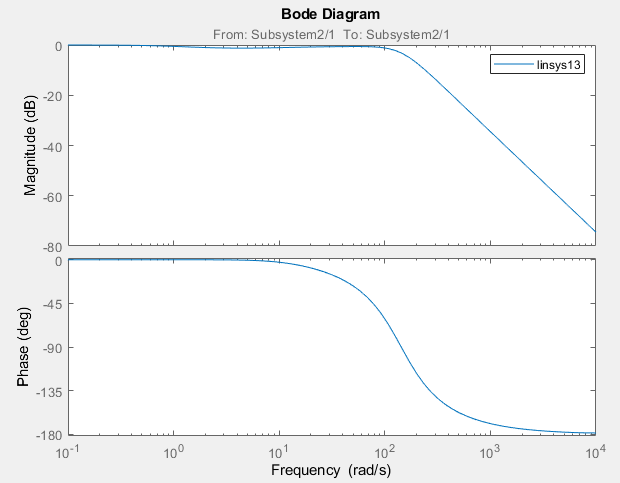
\includegraphics[width=0.8\linewidth]{Imagenes/loopshaping/bode_cerrando_p}
	\caption{Respuesta en frecuencia entre la fuerza aplicada al carrito y la posición de este.}
	\label{bode_cerrando_p}
\end{figure}

Agregamos un cero en $-0.05 \ \frac{rad}{s}$ para brindar adelanto de fase a la izquierda de $0.8 \ \frac{rad}{seg}$. Además agregamos un polo rápido en $-100 \ \frac{rad}{s}$ para hacer el controlador realizable. Graficando la respuesta en frecuencia de la ganancia de lazo se obtiene ahora:

\begin{figure}[H]
	\centering
	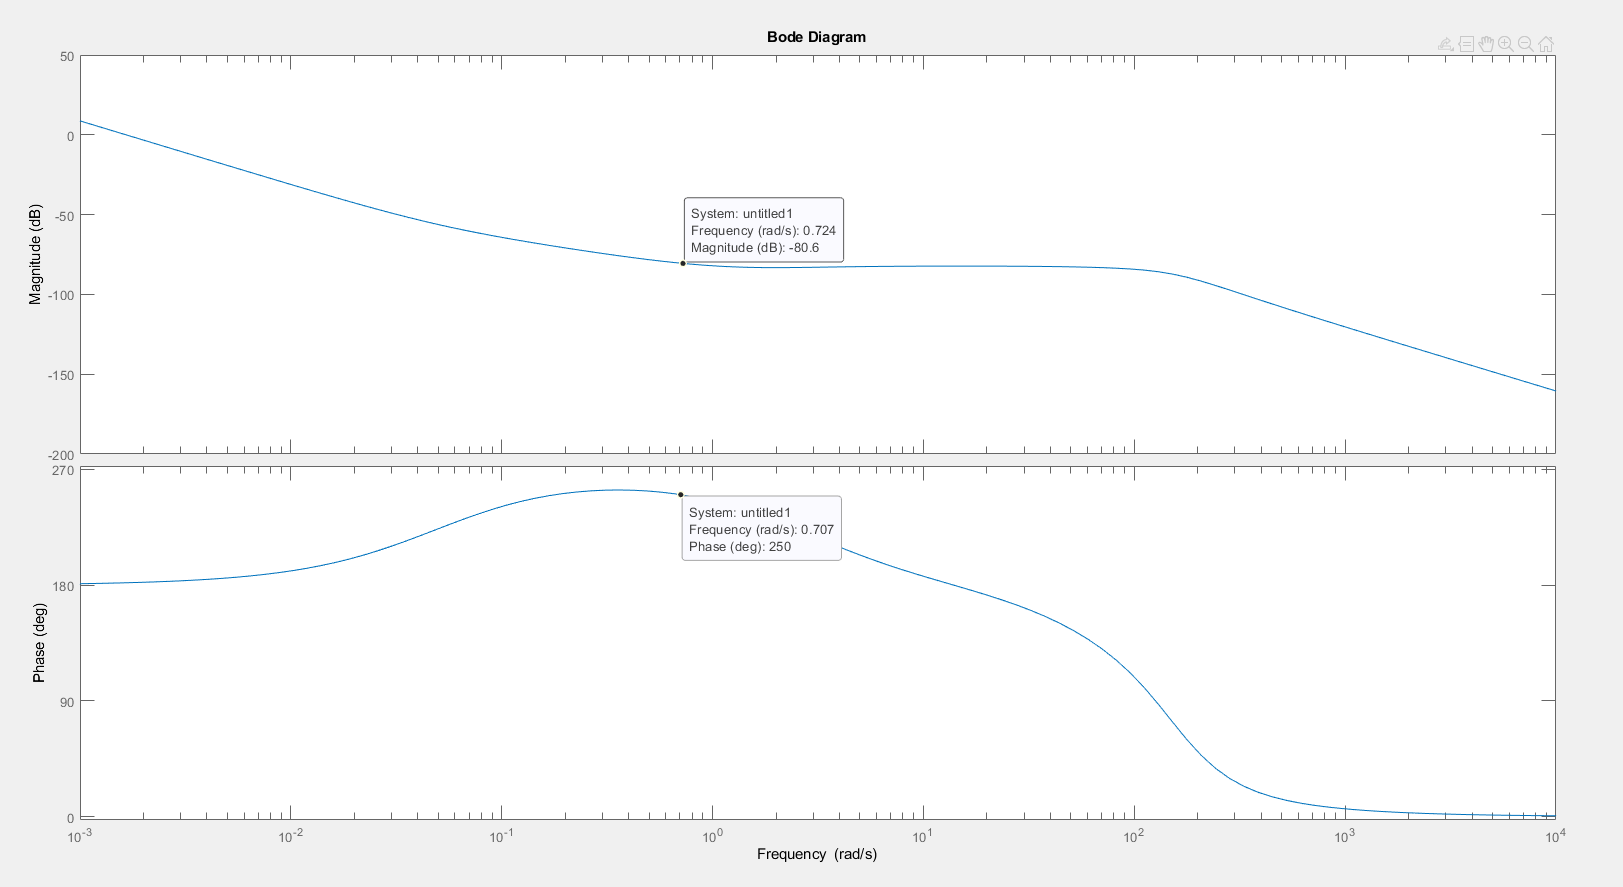
\includegraphics[width=0.8\linewidth]{Imagenes/loopshaping/bode_cerrando_p_con_controlador}
	\caption{Respuesta en frecuencia de la ganancia de lazo con controlador.}
	\label{bode_cerrando_p_con_controlador}
\end{figure}

Se agrega al controlador una ganancia de $80.6 \ dB$ para traer a la frecuencia de cruce a $0.7 \ \frac{rad}{s}$, por debajo del máximo impuesto por las limitaciones de diseño. Finalmente entonces se termina con

\begin{equation}
C_1(s) = 1.0715e+04 \cdot \frac{s+0.05}{s+100}
\end{equation}

y un margen de fase de $60$ grados.

Luego, se simula la respuesta del carrito como se observa en la Figura (\ref{simulacion_final}) ante una entrada del tipo step, obteniendo:

\begin{figure}[H]
	\centering
	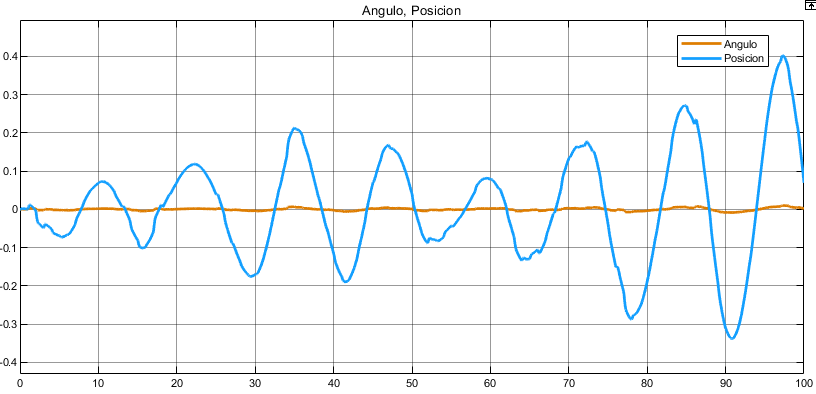
\includegraphics[width=0.8\linewidth]{Imagenes/loopshaping/simulacion_final}
	\caption{Simulación final de la planta controlando el ángulo del péndulo y la posición del carrito.}
	\label{simulacion_final}
\end{figure}

Finalmente, se discretiza el control utilizando el método de Tustin y colocando retensores de orden cero a la entrada y salida de la planta con una tasa de muestreo de $25 \ ms$, y se simula nuevamente, obteniendo:

 \begin{figure}[H]
	\centering
	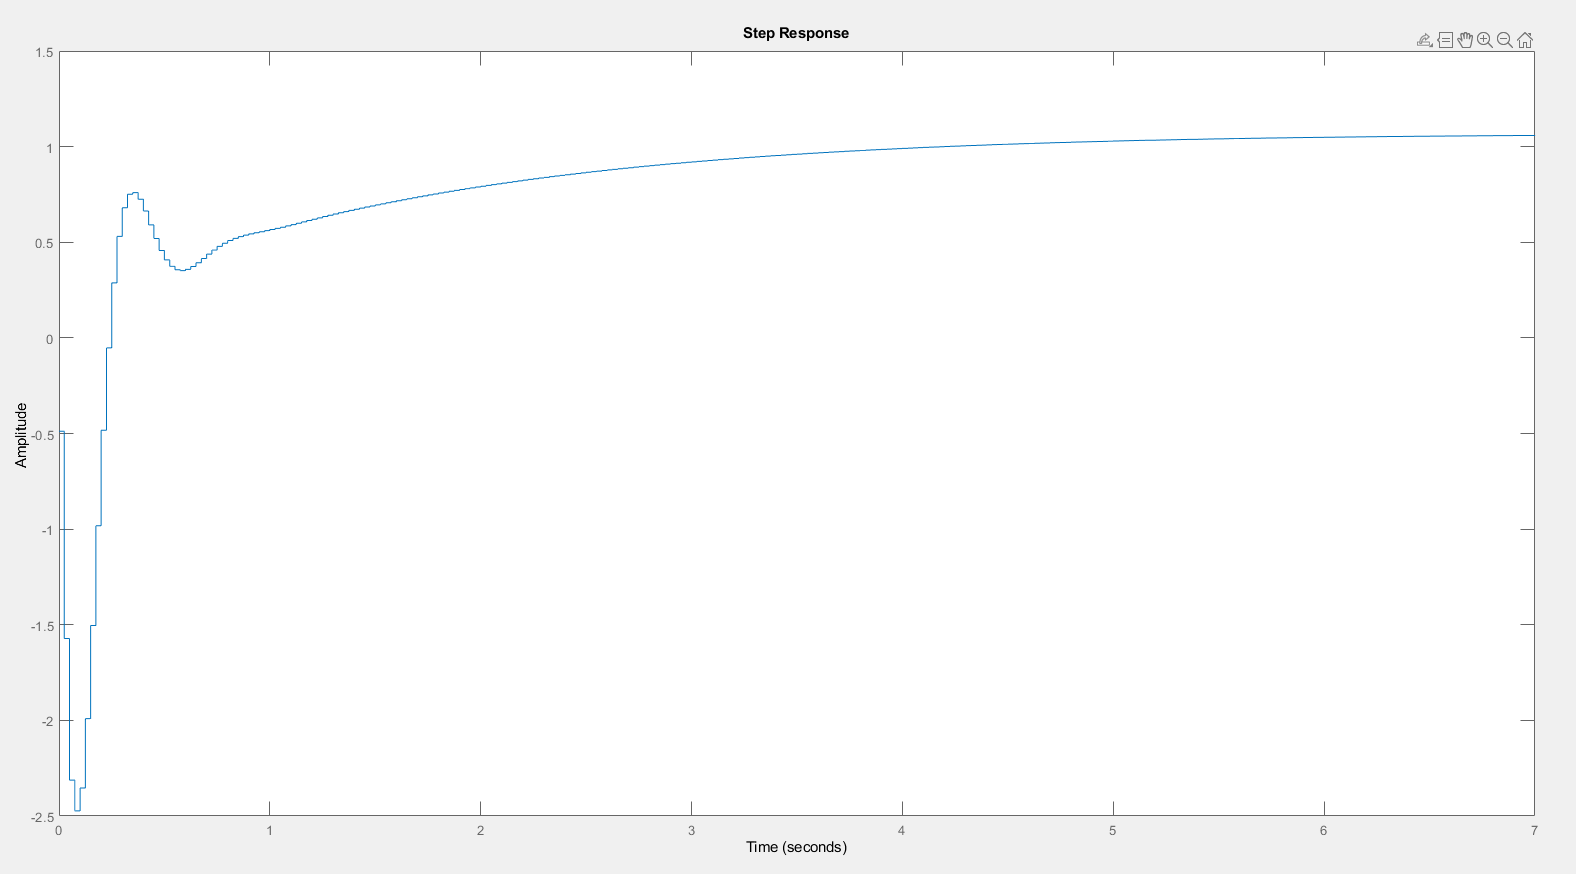
\includegraphics[width=0.8\linewidth]{Imagenes/loopshaping/simulacion_final_disc}
	\caption{Simulación discreta final de la planta controlando el ángulo del péndulo y la posición del carrito.}
	\label{simulacion_solo_angulo_disc}
\end{figure}


\section{Carro con Péndulo Simple: Control por realimentaci\'on de estados.}
\subsection{Perturbaciones}
Para las perturbaciones y cambios en la referencia se utiliz\'o el siguiente esquema:
Para los cambios de referencia se suma un escalón a la posici\'on de la planta. Para las perturbaciones en la mayoría de los casos se sumó a la acci\'on de control un tren de pulsos.
\begin{figure}[H]
	\centering
	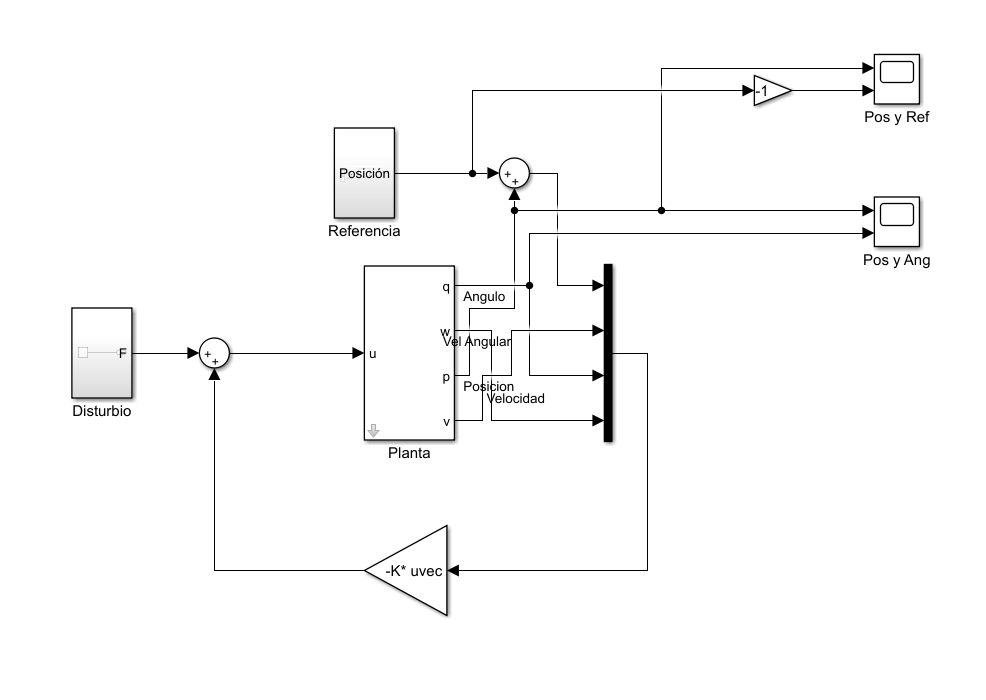
\includegraphics[width=1\linewidth]{Imagenes/Esquema_general.png}
	\caption{Esquema de perturbaciones y referencia.}
	\label{esq}
\end{figure}

Cabe notar que se utilizó un pasa-bajos en el camino de la referencia de posición a modo de pre-filtro para no desequilibrar demasiado al péndulo y apartarse demasiado del punto de linealización del sistema.

\subsection{Par\'ametros del modelo}
Linealizando al modelo mediante el uso del Linearizer de Simulink como descrito anteriormente, se obtuvieron las siguientes matrices que describen al sistema:
\begin{equation*}
A = 
\begin{pmatrix}
0 &  1 & 0 & 0 \\
0 &  0 & 1.7292 & 0 \\
0  & 0 & 0 & 1  \\
0 &  0 & 2.1615 & 0 
\end{pmatrix}
\end{equation*}

\begin{equation*}
B = 
\begin{pmatrix}
0  \\
0.941  \\
0   \\
0.1763  
\end{pmatrix}
\end{equation*}
Además se definió la siguiente matriz de salida para el sistema.
\begin{equation*}
C = 
\begin{pmatrix}
0 & 0 & 1 & 0 \\
1 & 0 & 0 & 0 
\end{pmatrix}
\end{equation*}
\begin{equation*}
D = 
\begin{pmatrix}
0 \\
0 
\end{pmatrix}
\end{equation*}
 Se realizó el estudio de controlabilidad y observabilidad del sistema, probando que este es controlable y observable teniendo como salida el \'angulo y posici\'on del carrito.
 Se notó que no era observable el sistema teniendo únicamente como salida el ángulo del carrito. Por lo que se opt\'o por conocer tanto la posici\'on como el \'angulo.
 
 \subsection{Realimentaci\'on de estados}
 Teniendo en cuenta que es controlable se realizó una realimentaci\'on de estados colocando los polos del sistema de la siguiente manera:
 \begin{itemize}
 \item Polo doble en -3.
  \item Polo doble en -2.
\end{itemize}
utilizando el comando acker.
El esquema de referencias y perturbaciones para este caso es el siguiente: al segundo de simulación, se cambia la referencia de posición de $0 \ m$ a $5 \ m$. A los $12$ segundos se cambia la referencia de $5 \ m$ a $-5 \ m$. Finalmente, a los 25 segundos se introduce un tren de pulsos con periodo 3 segundos y amplitud 500.
En la siguiente imagen se pueden ver 4 señales. En el primer cuadro se observan la referencia y la posición del carrito, en el segundo el ángulo del péndulo y en el último las perturbaciones.
Se puede apreciar cómo al cambiar la referencia, la posición la sigue. Además, la introducción de las perturbaciones provoca cambios tanto en el ángulo como en la posición, pero estas vuelven rápidamente a su condición de equilibrio. 
\begin{figure}[H]
	\centering
	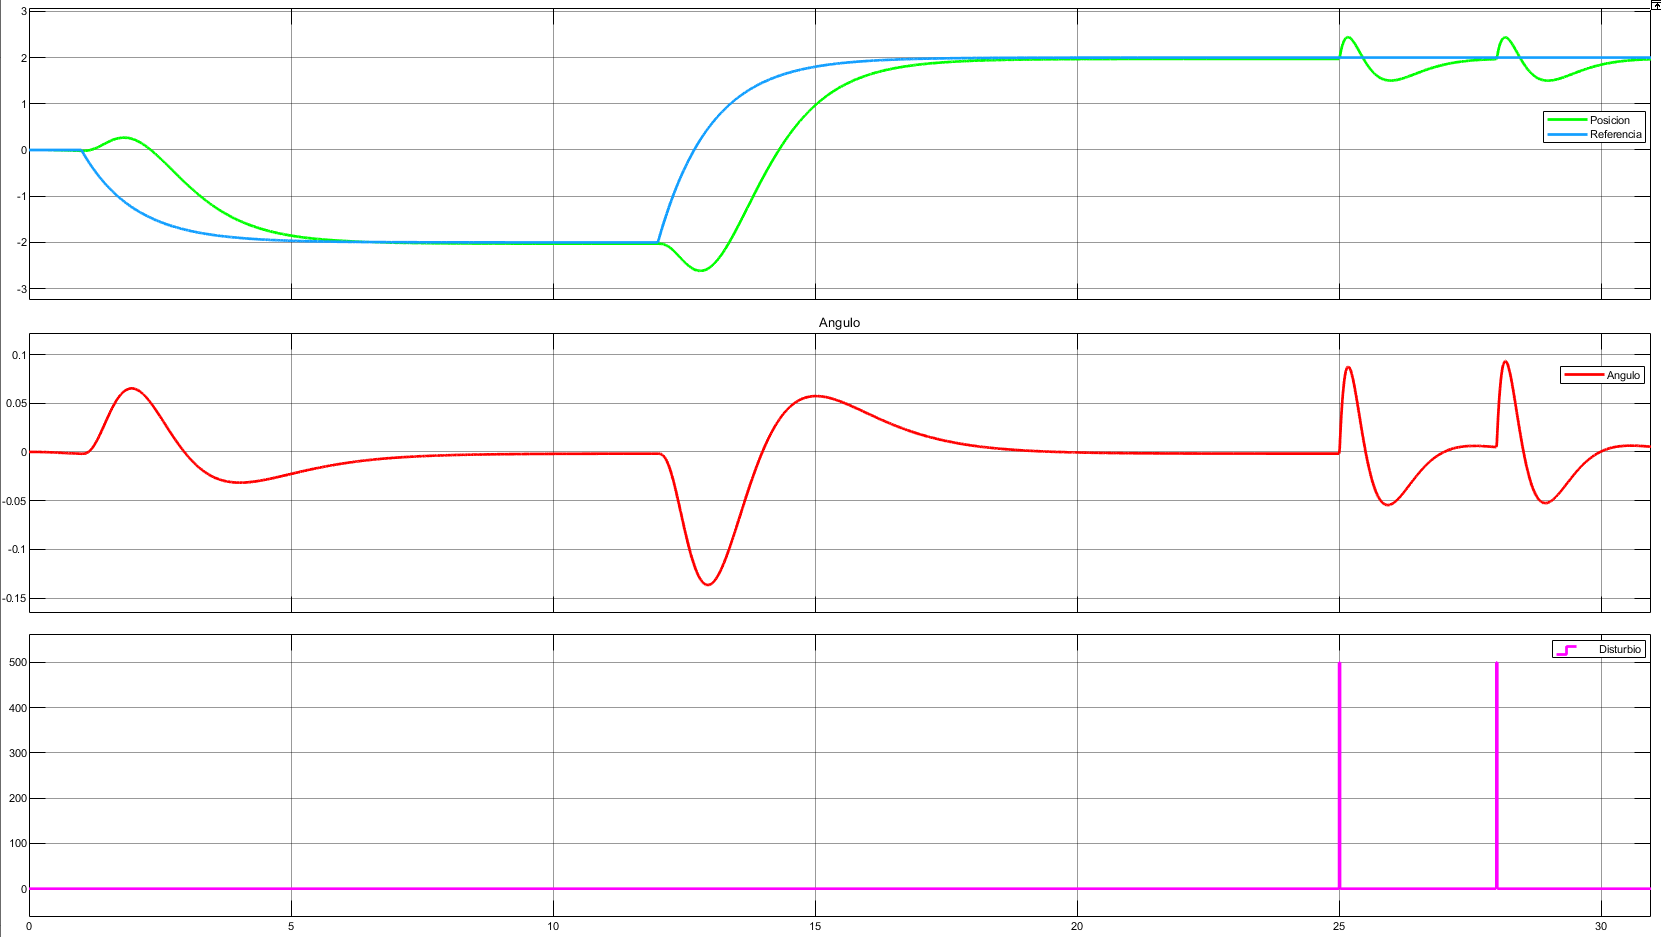
\includegraphics[width=1\linewidth]{Imagenes/Control_por_realimentacion/general.png}
	\caption{Respuesta del sistema a lazo cerrado.}
	\label{realmentacion}
\end{figure}

Aquí se puede observar que el sistema tiene error permanente. Esto se debe a que la planta no cuenta con acción integral para corregirlo.
\begin{figure}[H]
	\centering
	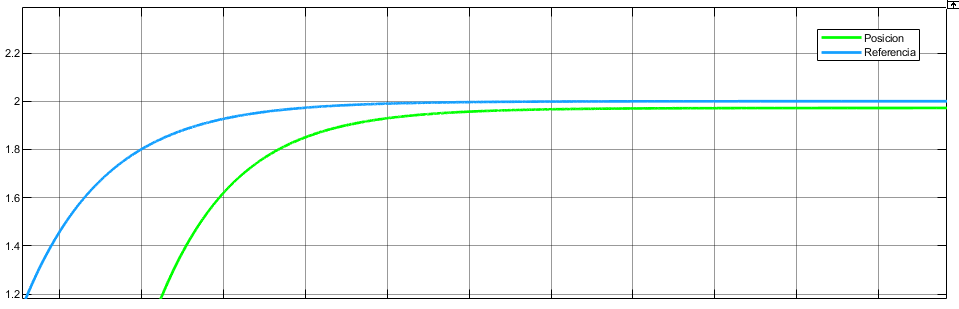
\includegraphics[width=1\linewidth]{Imagenes/Control_por_realimentacion/detalle_error_permanente.png}
	\caption{Detalle del error permanente.}
	\label{realmentacion_error}
\end{figure}

Así mismo se realizó un detalle en la interacción disturbio $\sim$ ángulo-posici\'on y cómo el sistema vuelve a la condici\'on de equilibrio.
\begin{figure}[H]
	\centering
	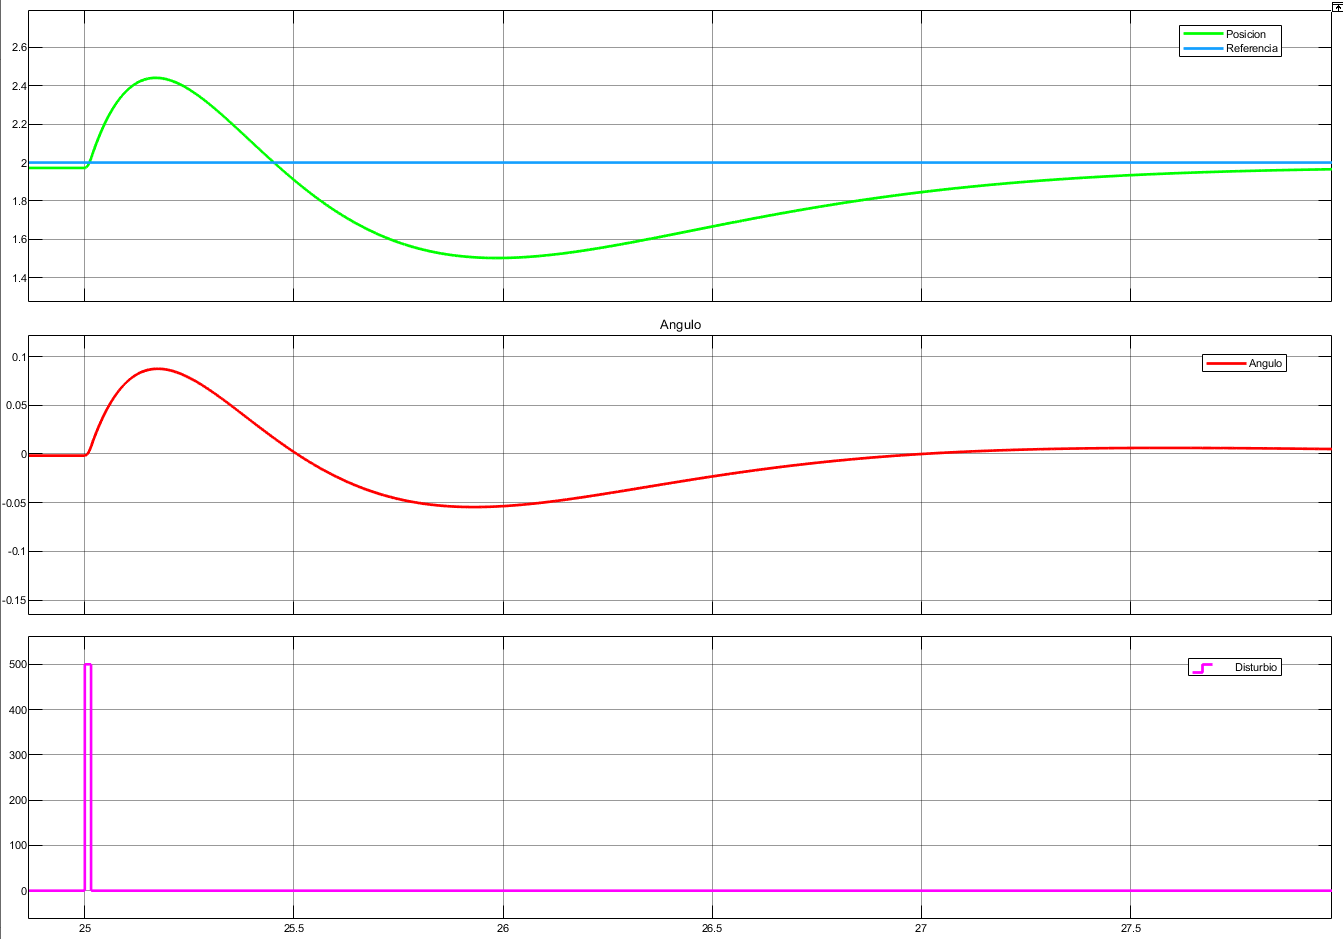
\includegraphics[width=1\linewidth]{Imagenes/Control_por_realimentacion/detalle_disturbio.png}
	\caption{Detalle disturbios.}
	\label{realmentacion_disturbio}
\end{figure}


 \subsection{Realimentaci\'on de estados con observador discreto}
Finalmente se diseñó un observador discreto de estados para el sistema. Para el observador se consideraron polos por lo menos una década mas rápidos que los de la planta, para garantizar rápida convergencia a cero del error entre salidas.
Además, se eligi\'o un valor para el tiempo de muestreo. Para esto se busco un tiempo que sea lo más alto posible y que funcione correctamente el control. Para este caso en particular fue $T_s=0.1 \ s$.
Se propuso el siguiente esquema de control:
\begin{figure}[H]
	\centering
	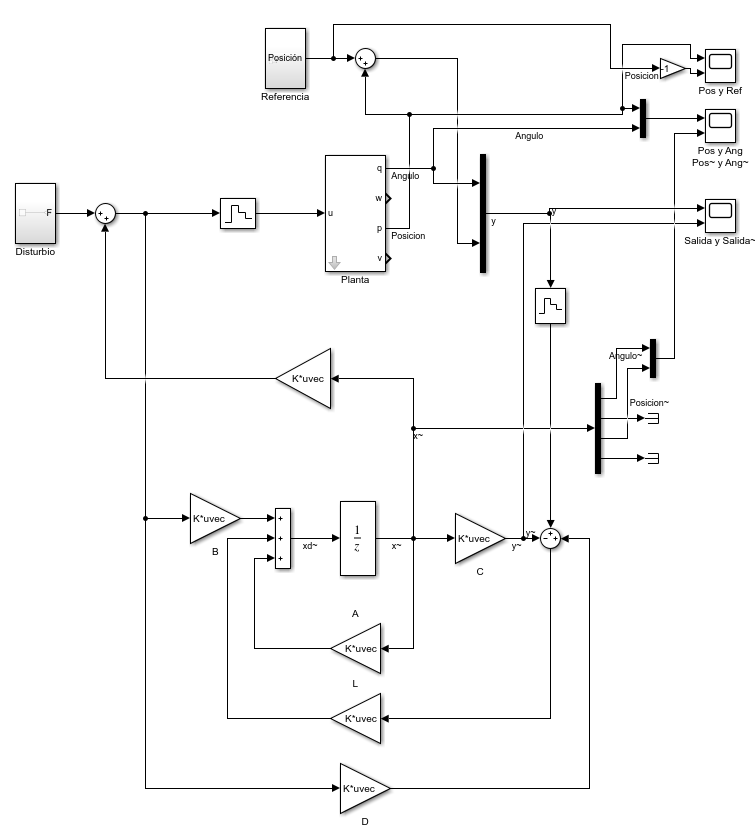
\includegraphics[width=1\linewidth]{Imagenes/Esquema_general_obs_disc.png}
	\caption{Esquema de control de realimentación de estados con observador discreto.}
	\label{esqdisctobs}
\end{figure}

En estas mediciones se puede observar que además se agregó una señal que es la discreta, luego del sample and hold.
Se puede apreciar en este caso también cómo al cambiar la referencia la posición sigue a la misma, y además cómo la introducción de las perturbaciones provoca cambios tanto en el ángulo como en la posición, pero estas vuelven rápidamente a su condición de equilibrio. 
\begin{figure}[H]
	\centering
	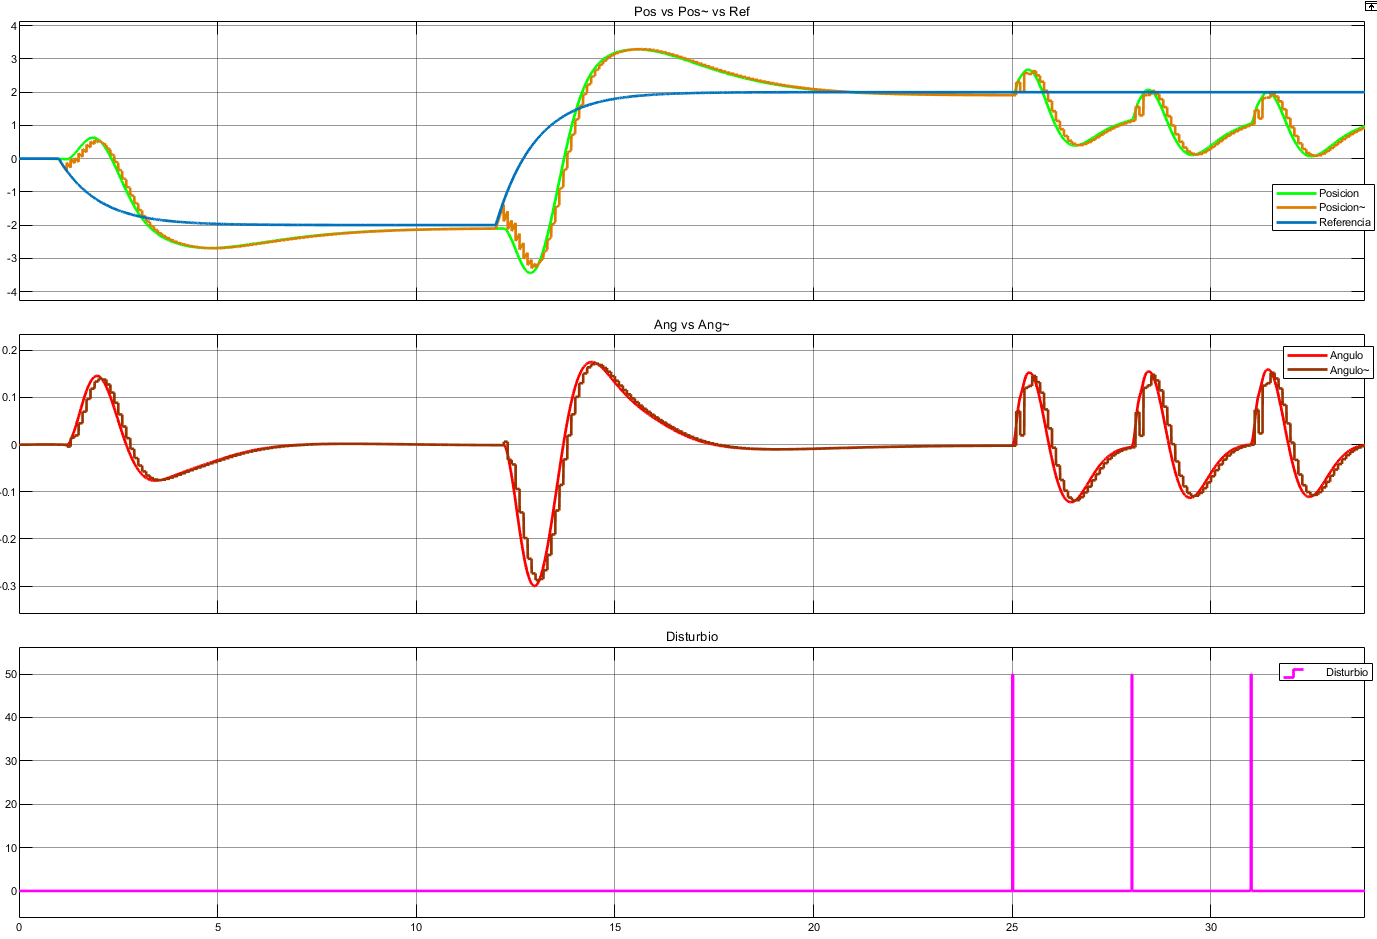
\includegraphics[width=1\linewidth]{Imagenes/Control_Obs_Discreto/general.png}
	\caption{Respuesta del sistema con realimentación de estados y observador discreto a lazo cerrado.}
	\label{realmentacion}
\end{figure}

Se observa claramente la diferencia entre la señal de posición real, la discreta y la referencia deseada, al igual de cómo las tres convergen al mismo punto.
\begin{figure}[H]
	\centering
	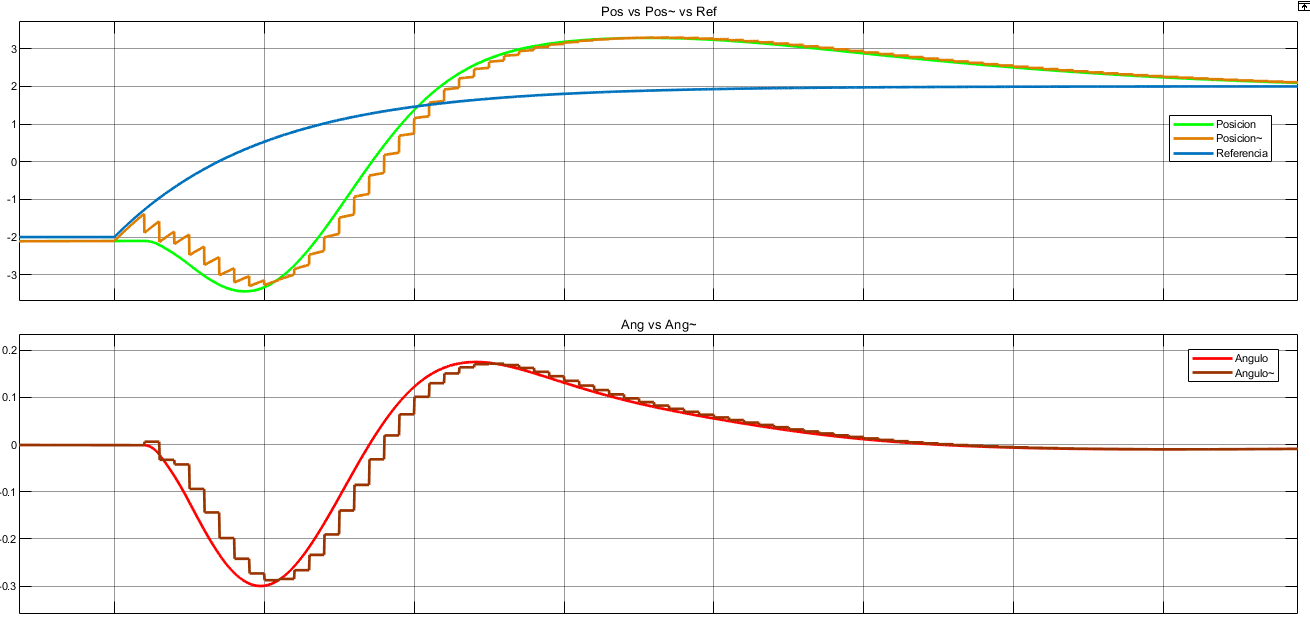
\includegraphics[width=1\linewidth]{Imagenes/Control_Obs_Discreto/detalle_angulo_pos.png}
	\caption{Detalle \'angulo posición.}
	\label{realmentacion_error}
\end{figure}

Agregamos finalmente esta imagen para ver cómo la señal discreta coincide con la señal real cada Ts y cómo teniendo una frecuencia de muestreo tan chica aún se consigue un control eficaz.
\begin{figure}[H]
	\centering
	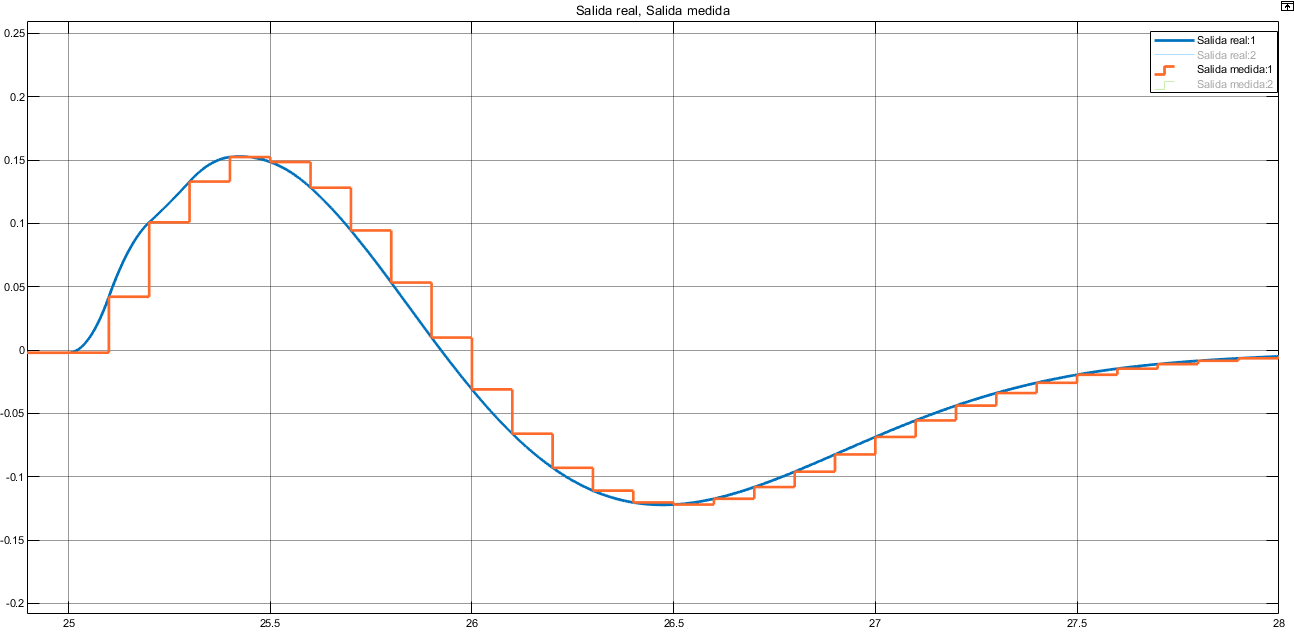
\includegraphics[width=1\linewidth]{Imagenes/Control_Obs_Discreto/detalle_real_medido.png}
	\caption{Detalle continuo discreto.}
	\label{realmentacion_disturbio}
\end{figure}


\subsection{Realimentaci\'on de estados con control integral}
Adicionalmente se realizó una realimentaci\'on de estados con control integral, teniendo como salida la posici\'on del carrito. Esto trae un problema el cual es que deja de ser observable el sistema, por lo que el sistema no podría realizarse con las salidas definidas, sino que habría que tener mayor información de las otras variables.
Se propuso el siguiente esquema de control:
\begin{figure}[H]
	\centering
	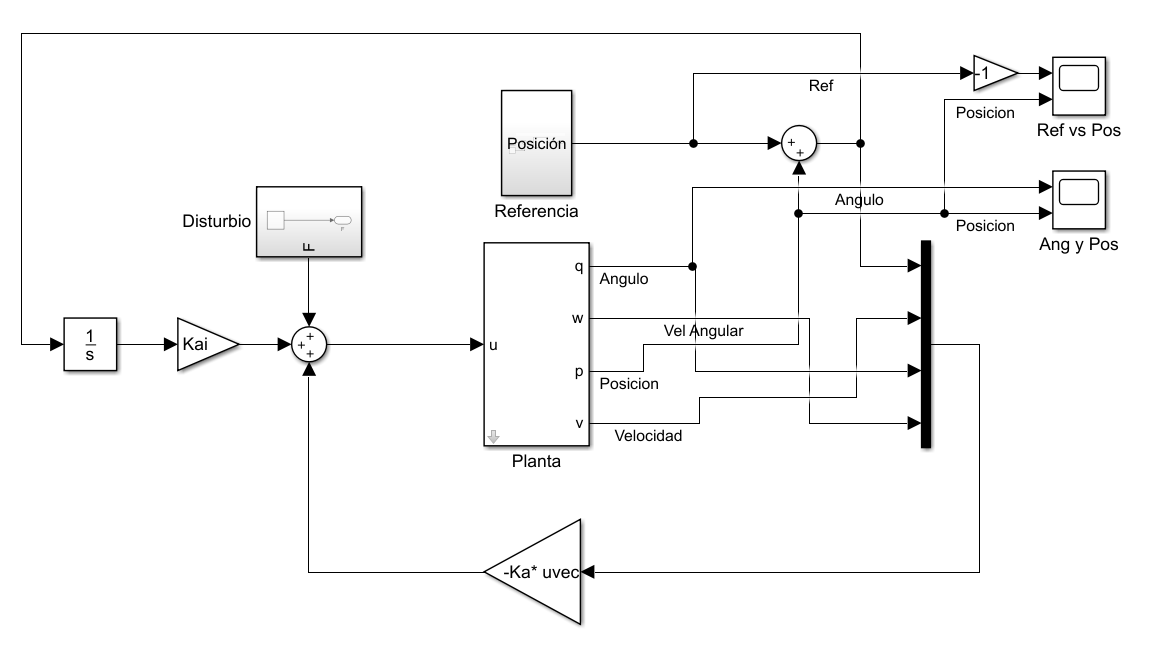
\includegraphics[width=1\linewidth]{Imagenes/Esquema_general_int.png}
	\caption{Esquema de control realimentación de estados con acción integral.}
	\label{esqint}
\end{figure}

Se puede apreciar cómo al cambiar la referencia la posición sigue al mismo, y ademas como la introducción de las perturbaciones provoca cambios tanto en el ángulo como en la posición, para volver rápidamente a la condición de equilibrio. 
\begin{figure}[H]
	\centering
	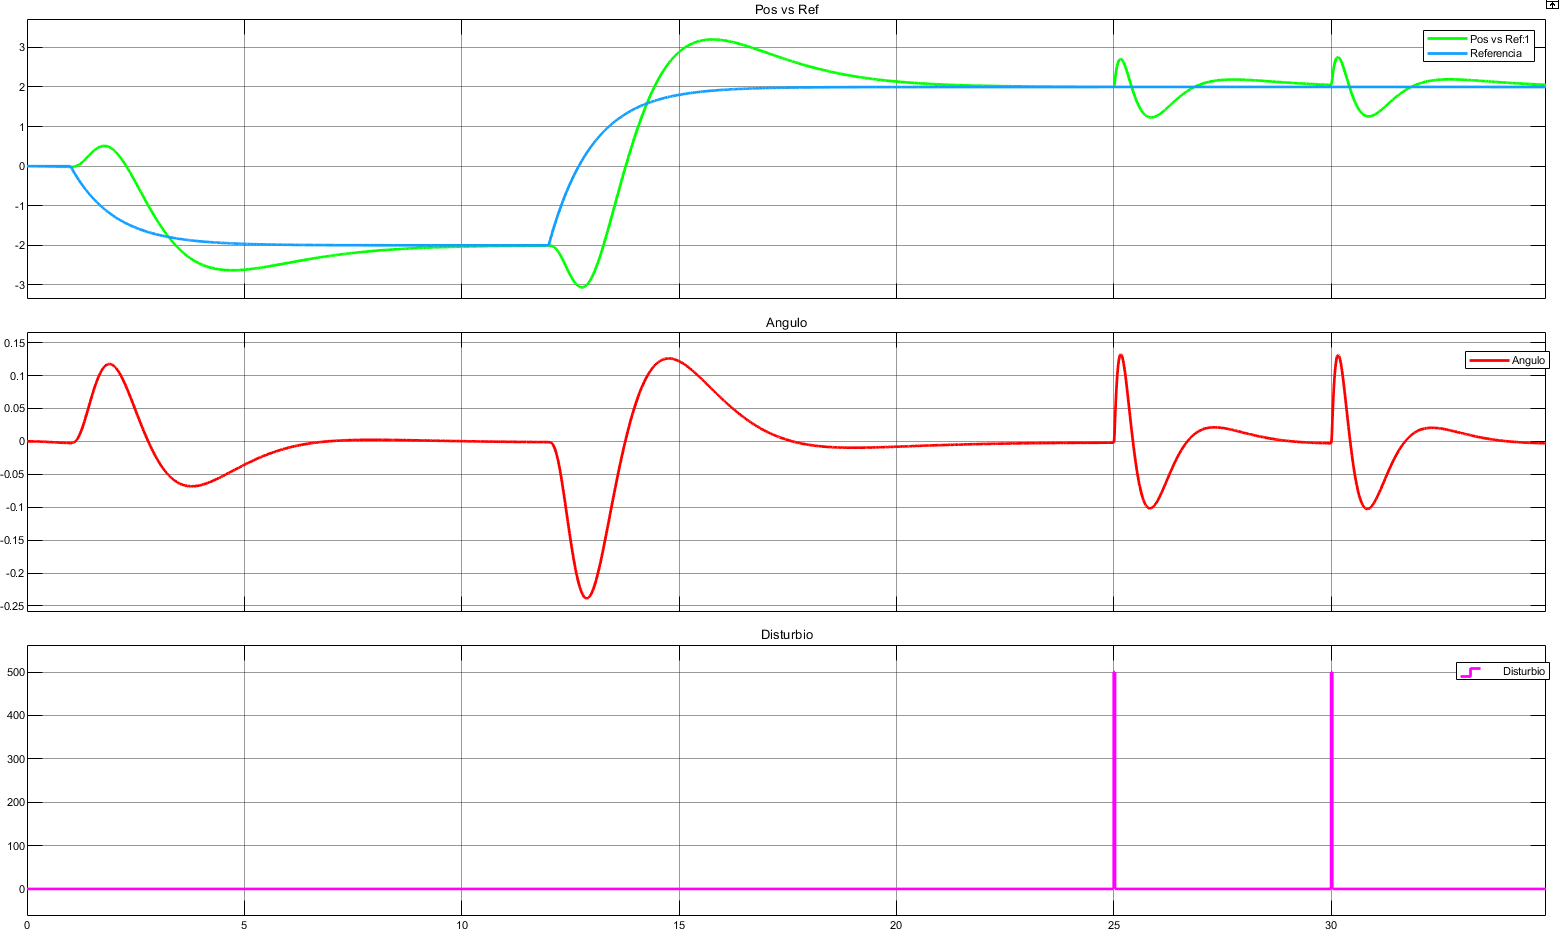
\includegraphics[width=1\linewidth]{Imagenes/Control_por_realimentacion_integral/general.png}
	\caption{Respuesta del sistema con realimentación de estados y control integral a lazo cerrado.}
	\label{realmentacion}
\end{figure}

Aquí se puede ver que a diferencia del sistema sin acci\'on integral este no tiene error permanente.
\begin{figure}[H]
	\centering
	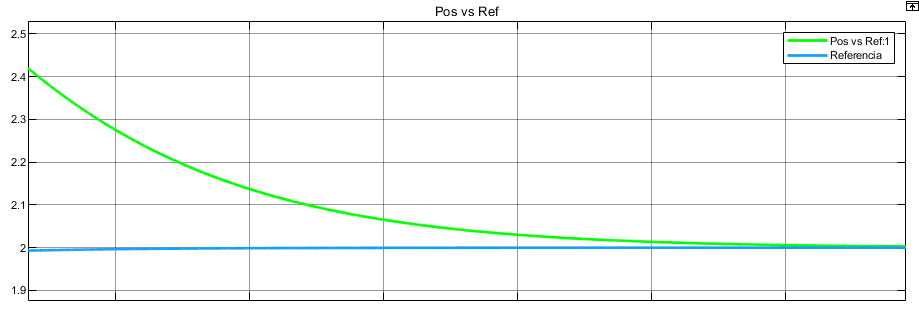
\includegraphics[width=1\linewidth]{Imagenes/Control_por_realimentacion_integral/detalle_error_permanente.png}
	\caption{Detalle error permanente.}
	\label{realmentacion_error}
\end{figure}

Así mismo se realizó un detalle en la interacción disturbio $\sim$ ángulo-posici\'on y cómo el sistema vuelve a la condici\'on de equilibrio.
\begin{figure}[H]
	\centering
	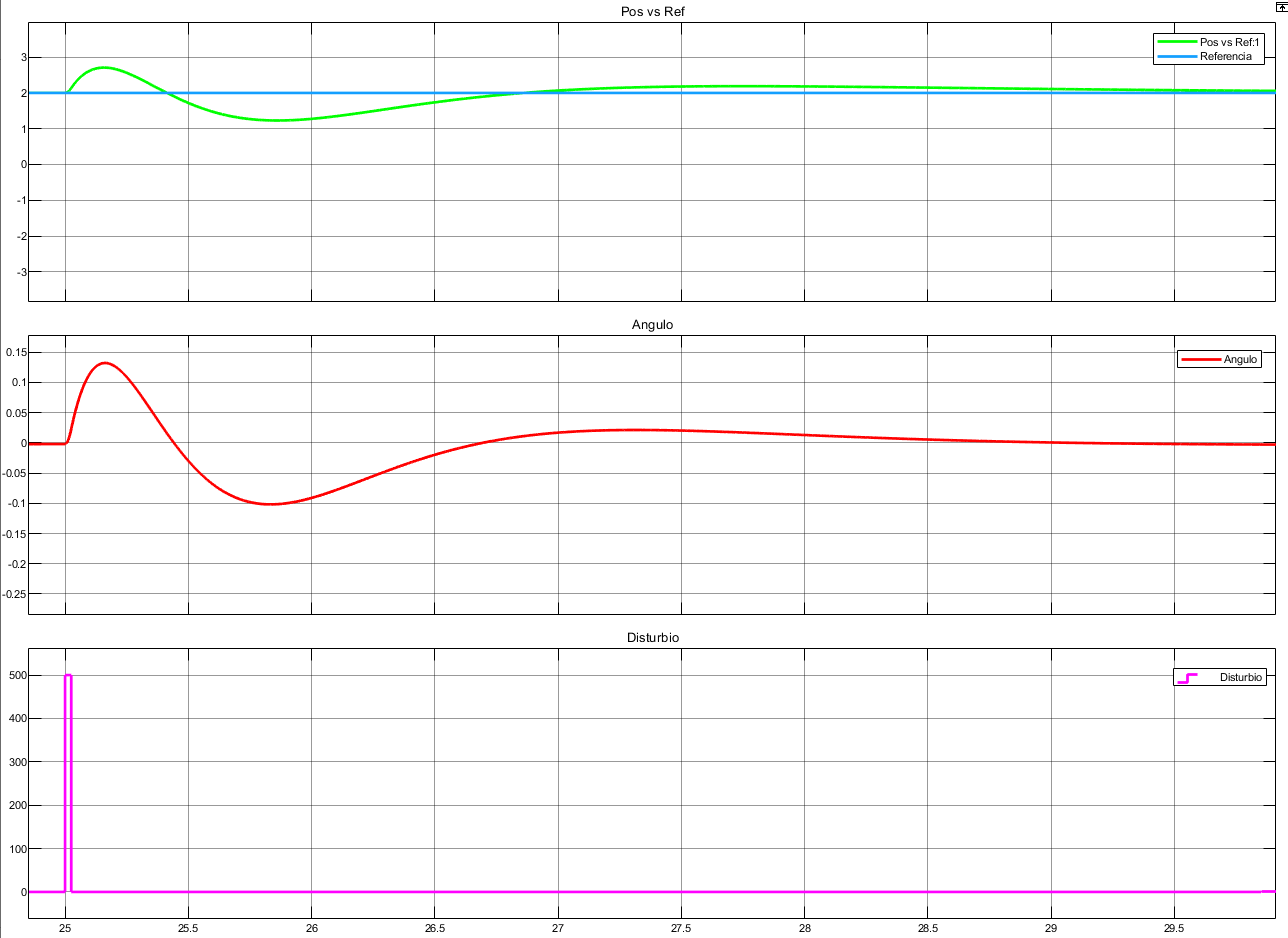
\includegraphics[width=1\linewidth]{Imagenes/Control_por_realimentacion_integral/detalle_disturbio.png}
	\caption{Detalle disturbios.}
	\label{realmentacion_disturbio}
\end{figure}

\subsection{Realimentaci\'on de estados con control integral en tiempo discreto}
A continuaci\'on se discretiz\'o el sistema a través de la transformada de Tustin. Obteniendo los siguientes resultados:

\begin{figure}[H]
	\centering
	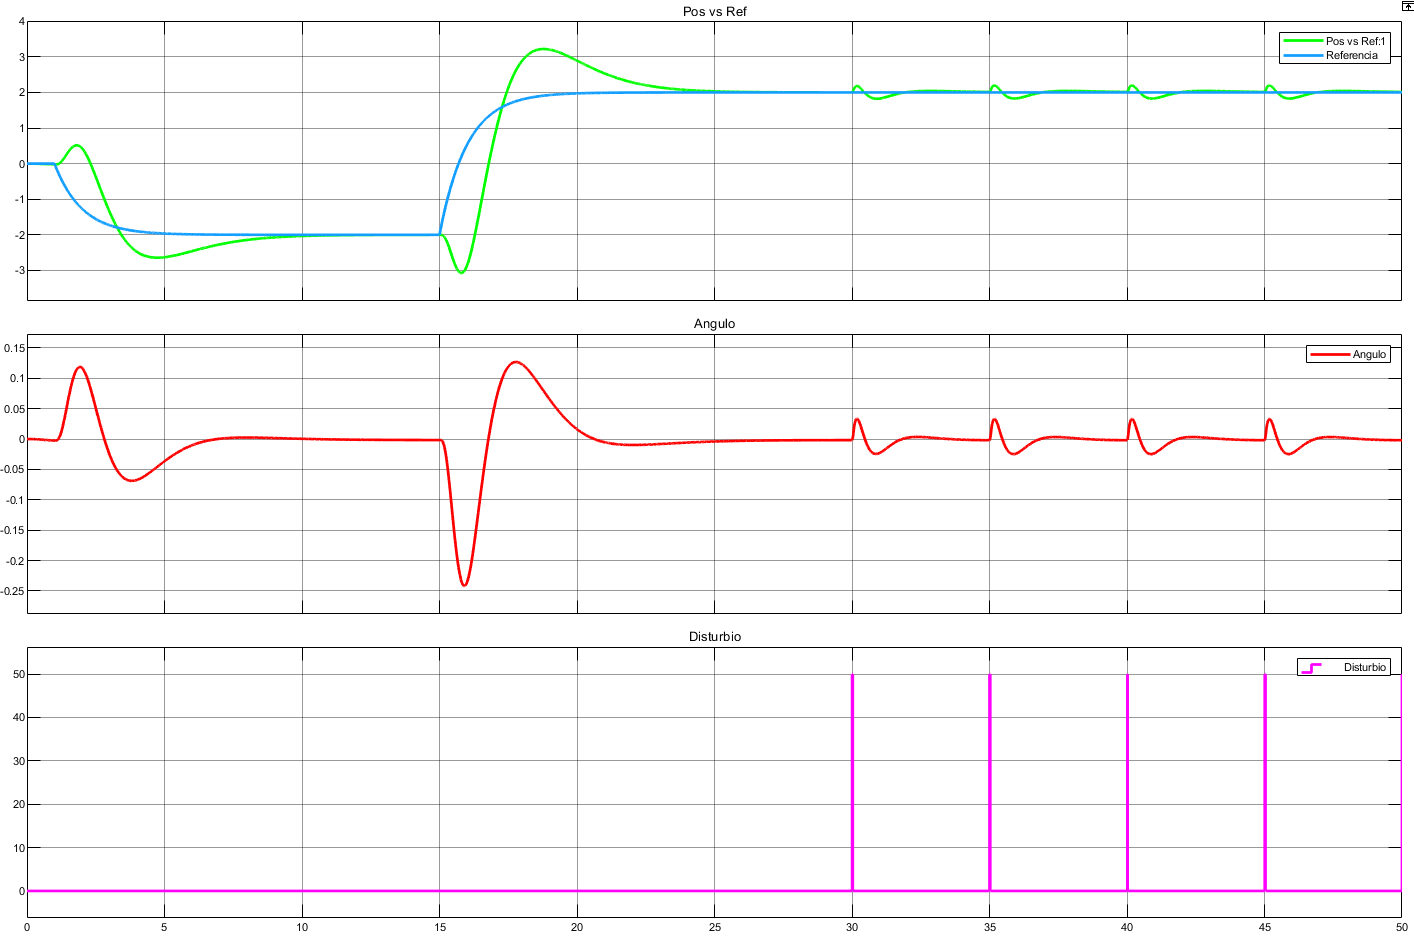
\includegraphics[width=1\linewidth]{Imagenes/Control_integral_disc/general.png}
	\caption{Respuesta del sistema a lazo cerrado.}
	\label{realmentacion}
\end{figure}

Aquí se puede ver que a diferencia del sistema sin acci\'on integral este tampoco no tiene error permanente.
\begin{figure}[H]
	\centering
	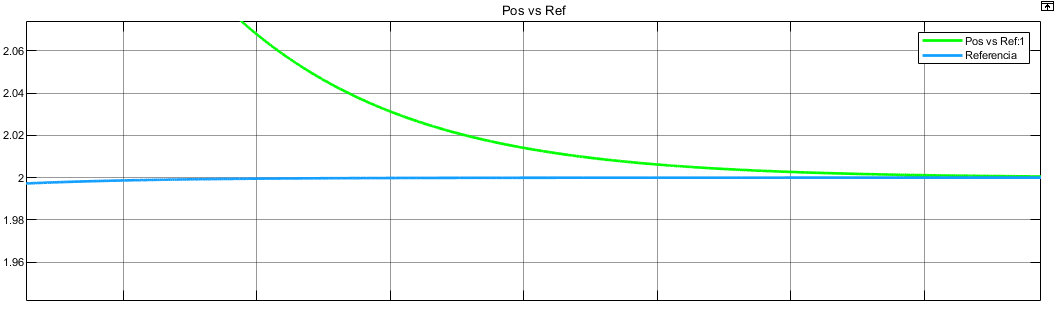
\includegraphics[width=1\linewidth]{Imagenes/Control_integral_disc/detalle_error_permanente.png}
	\caption{Detalle error permanente.}
	\label{realmentacion_error}
\end{figure}

Así mismo se realizó un detalle en la interacción disturbio $\sim$ ángulo-posici\'on y como el sistema vuelve a la condici\'on de equilibrio.
\begin{figure}[H]
	\centering
	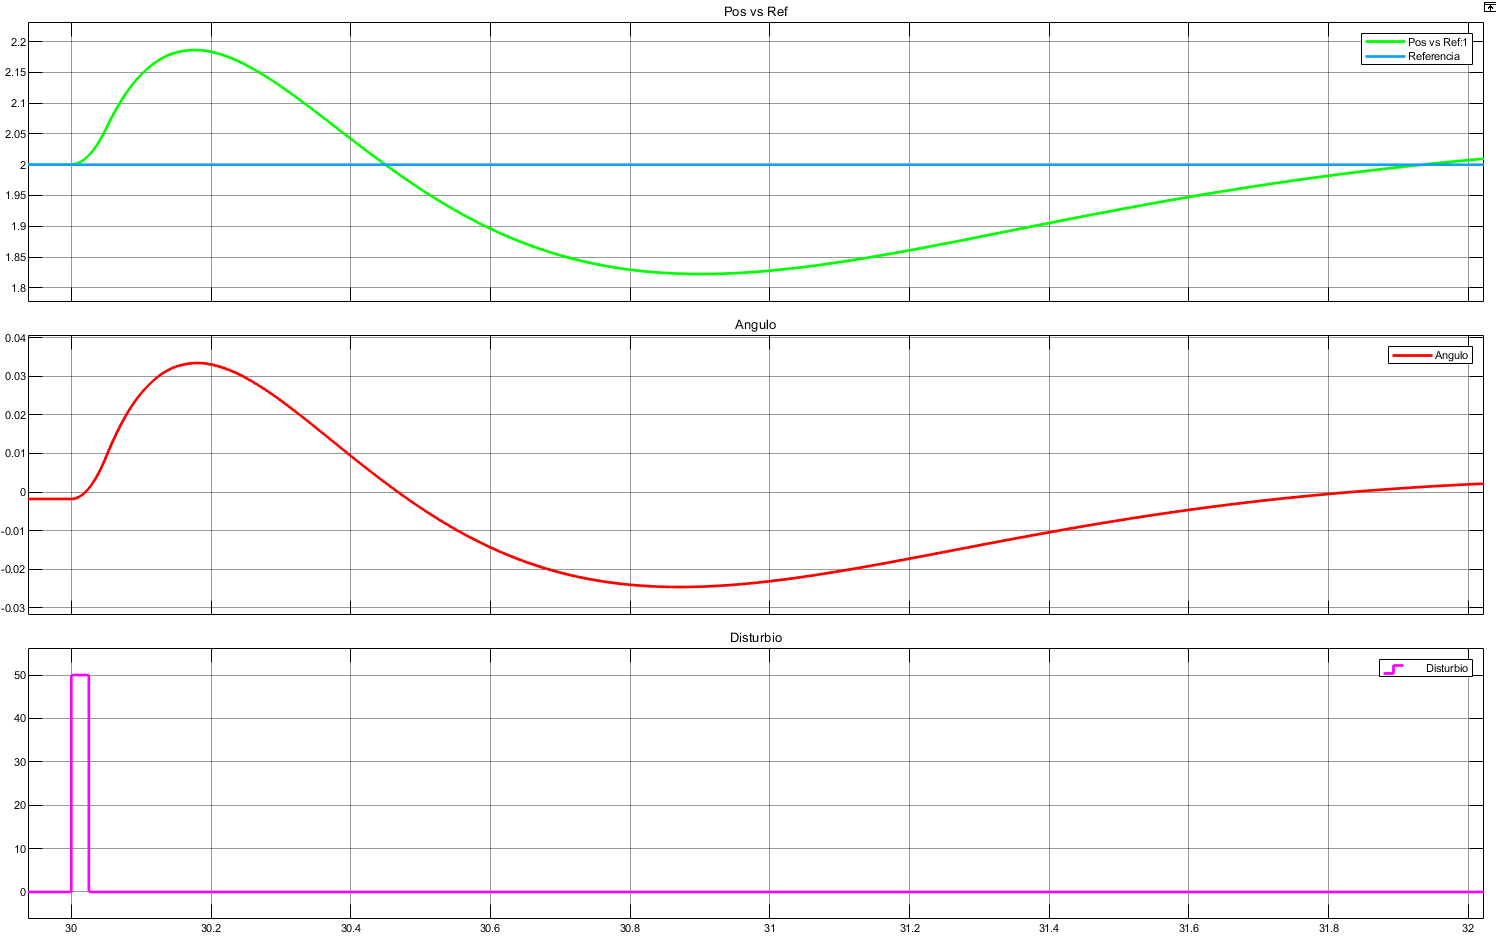
\includegraphics[width=1\linewidth]{Imagenes/Control_integral_disc/detalle_disturbio.png}
	\caption{Detalle disturbios.}
	\label{realmentacion_disturbio}
\end{figure}

\begin{figure}[H]
	\centering
	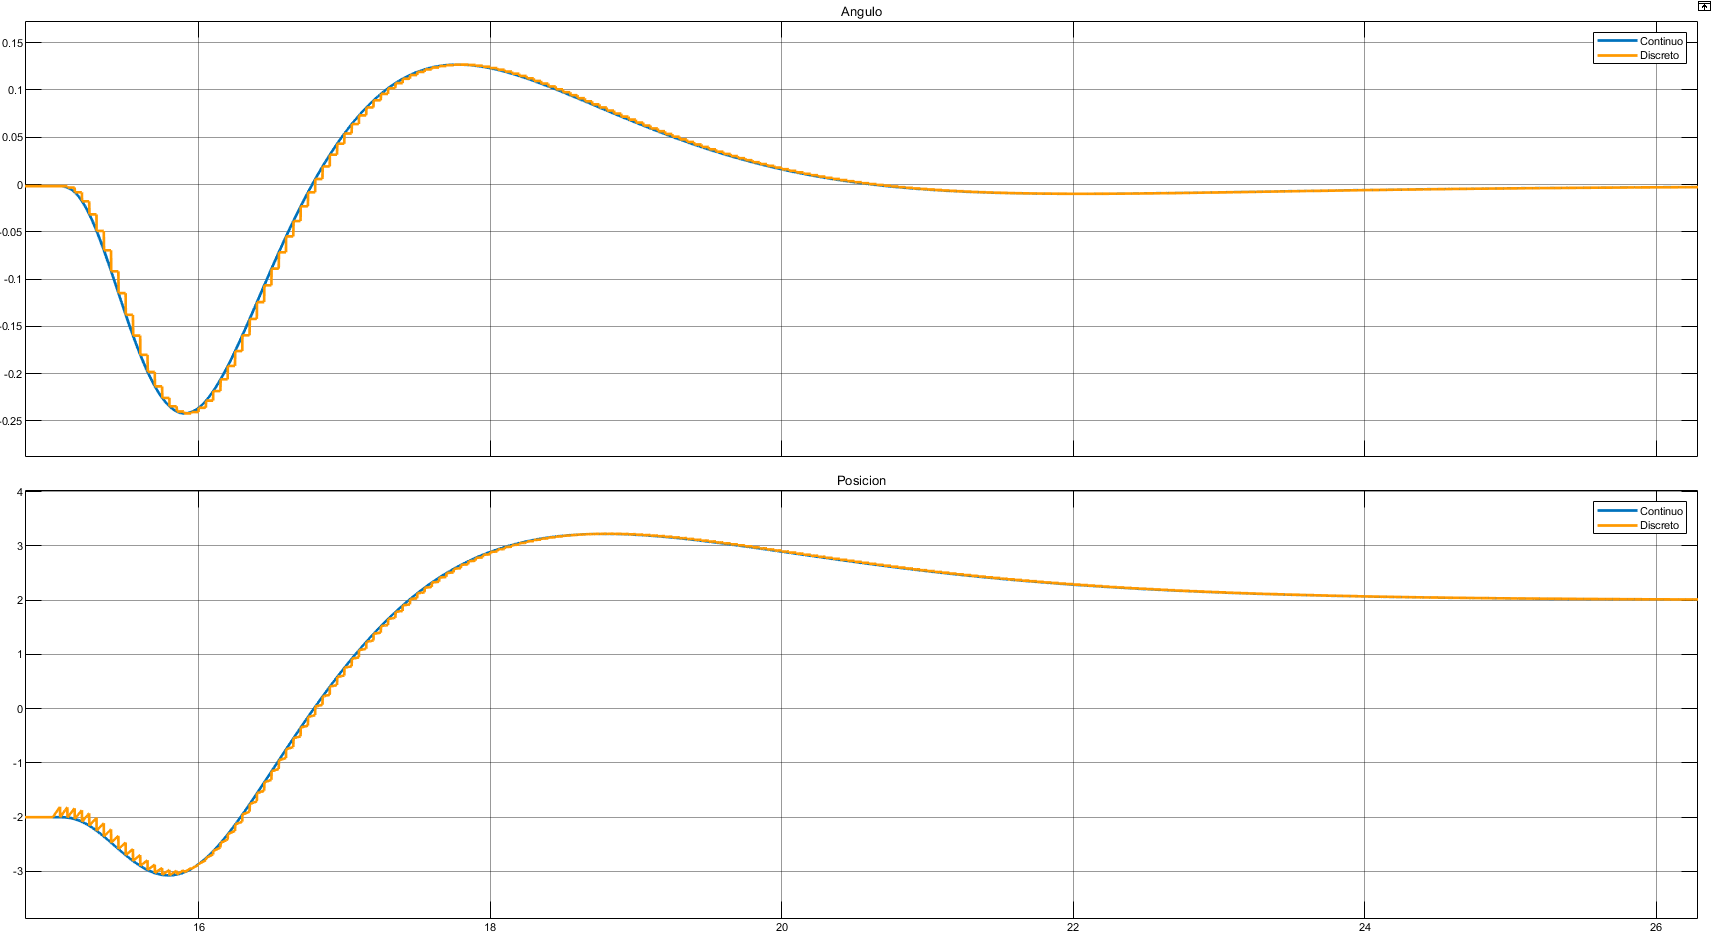
\includegraphics[width=1\linewidth]{Imagenes/Control_integral_disc/detalle_real_medido.png}
	\caption{Detalle continuo discreto.}
	\label{realmentacion_disturbio}
\end{figure}

\section{Conclusiones}

Se realizó un control por loop shaping enfrentándonos a varias dificultades. Por un lado, la planta tenía un polo en el semiplano derecho, lo que limitaba inferiormente al ancho de banda del controlador del primer lazo, teniendo que hacer a este control lo suficientemente rápido para que venza esta alinealidad. Por otro lado, para el caso de la posición, la planta tenía un cero en el semiplano derecho lo que limitaba superiormente a la velocidad del controlador del segundo lazo. Esto tiene sentido, dado que si se busca achicar el error con la referencia de posición demasiado rápido, se puede llegar a perder la condición de linealidad en la cercanía del equilibrio al desplazar de manera demasiado brusca el ángulo del péndulo. 

Luego, se realizaron controles por realimentación de estados, sin y con observador discreto al igual que un control con acción integral. También se realizaron estudios de observabilidad y controlabilidad, que fijaron qué salidas debería tener el sistema para poder realizar un observador en cada caso, dado que no todos los sistemas eran observables.

Una observación interesante es la del efecto del cero en el semiplano derecho en la respuesta transitoria del sistema. Esta alinealidad provoca que, ante un cambio en la referencia de posición, el control procede a desplazar el carrito hacia el lado contrario de la nueva referencia para luego sí desplazarse hacia ella. Esto tiene sentido, dado que si se desea desplazar al carrito hacia la derecha, primero se debe desbalancear al péndulo hacia esta dirección, lo cual se logra moviendo al carro primero hacia la izquierda.

La mayor discrepancia entre ambos tipos de controles implementados, por loop shaping y por realimentación de estados, se da en la calidad del control y la respuesta transitoria que se obtiene. Esto se debe a que para el caso de loop shaping, solamente se puede realimentar la posición y el ángulo, tratándolos de manera independiente, mientras que para la realimentación de estados se pueden realimentar todos los estados y fijar los polos donde se desea, a costo de un control mucho más complejo.
\end{document}
